% 菲涅尔公式 布儒斯特角
% 菲涅尔|折射|反射|偏振|布儒斯特角

\pentry{麦克斯韦方程组(介质)\upref{MWEq1}}

\begin{figure}[ht]
\centering
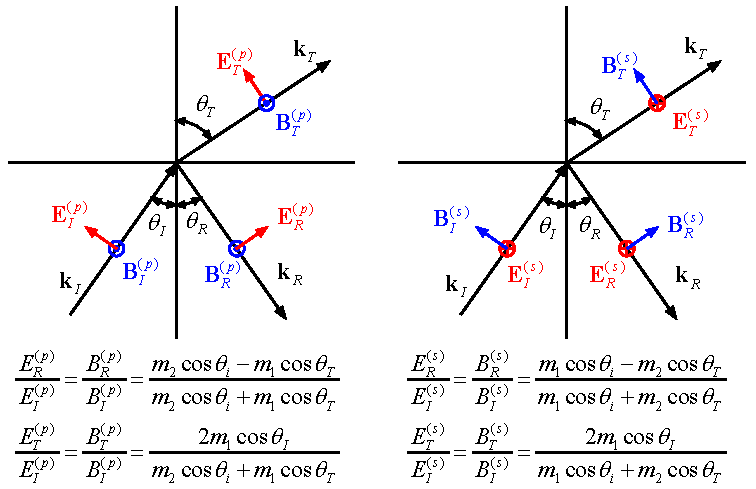
\includegraphics[width=14cm]{./figures/Fresnl_1.pdf}
\caption{菲涅尔公式} \label{Fresnl_fig1}
\end{figure}
 
利用具体的电磁场的边界条件 % 链接未完成
\begin{itemize}
\item $\div \bvec D = 0$ 和$\div \bvec B = 0$  分别对应 $\epsilon \bvec E_\bot = \epsilon' \bvec E'_\bot$ 和 $\epsilon \bvec B_\bot = \epsilon' \bvec B'_\bot$.

\item $\div \bvec E = 0$ 和 $\div \bvec H = 0$ 分别对应 $\bvec E_{//} = \bvec E'_{//}$ 和 $\bvec B_{//}/\mu = \bvec B'_{//}/\mu'$.
\end{itemize}

现在分两种情况讨论
\begin{enumerate}
\item 极化方向垂直于入射面(\autoref{Fresnl_fig1} 右)

\begin{equation}
\frac{E_R^{(s)}}{E_I^{(s)}} =  \frac{m_1\cos{\theta_I} - m_2\cos\theta_T}{m_1\cos\theta_I + m_2\cos\theta_T}
\qquad
\frac{E_T^{(s)}}{E_I^{(s)}} = \frac{2 m_1\cos\theta_I}{m_1\cos\theta_I + m_2\cos\theta_T}
\end{equation}

\item 极化方向平行于入射面(\autoref{Fresnl_fig1} 左)
\begin{equation}\label{Fresnl_eq2}
\frac{E_R^{(p)}}{E_I^{(p)}} =  \frac{m_2\cos\theta_I - m_1\cos\theta_T}{m_2 \cos\theta_I + m_1\cos\theta_T}
\qquad
\frac{E_T^{(p)}}{E_I^{(p)}} =  \frac{2 m_1\cos\theta_I}{m_2\cos\theta_I + m_1\cos\theta_T}
\end{equation}
\end{enumerate}
其中 $m_I=n_I/\mu_I = c\sqrt{\epsilon_I/\mu_I}$, 一般情况下介质的磁导率于真空区磁导率的区别可忽略,即可以把 $m_I$ 替换为折射率 $n_I$. 另外注意菲涅尔公式包含相位信息,即以上的 $E$ 可以是复振幅.

\subsection{布儒斯特角}
我们这里考虑常见的 $n_2>n_1$ 且 $\mu_1 = \mu_2$ 情况.由\autoref{Fresnl_eq2} 容易证明当入射角为\textbf{布儒斯特角(Brewster's angle)} 时反射光的平行(p)分量消失.布儒斯特角等于
\begin{equation}
\theta_B = \arctan (n_2/n_1)
\end{equation}
% 未完成: 画图!